\documentclass[aspectratio=169]{beamer}
\mode<presentation> {
\usetheme{default}
\usecolortheme{dolphin}
}
\usepackage{algorithm,algorithmic}
\usepackage{caption}
\usepackage{multirow}
\usepackage{threeparttable}
\usepackage{natbib}
\bibliographystyle{aer}
\usepackage{graphicx}
\usepackage{parskip}
\usepackage{float}
\usepackage{alphabeta}
\usepackage{multirow,array}
\usepackage{subfig}
\usepackage{amsmath}
\usepackage{amssymb}
\usepackage{mathabx}
\usepackage{caption}
\usepackage{pifont} 
\usepackage{booktabs,tabularx}
\newcolumntype{Y}{>{\raggedright\arraybackslash}X}

\usepackage{tikz}
\usetikzlibrary{arrows.meta,positioning,calc,fit,backgrounds,decorations.pathreplacing, shapes.geometric}
\graphicspath{{figures/}}
\usetikzlibrary{matrix,chains,positioning,decorations.pathreplacing,arrows}

% TikZ Styles - Adjusted font sizes for clarity since bold is removed
\tikzset{
  >=Stealth,
  st/.style={circle,draw,inner sep=0pt,minimum size=6mm, fill=white}, 
  action/.style={circle,fill=black,inner sep=0pt,minimum size=2mm},
  tr/.style={-Stealth, line width=0.8pt},
  lbl/.style={font=\footnotesize},
  block/.style={rectangle, draw, fill=blue!10, rounded corners, minimum height=2em}
}

\newcommand{\E}{\mathbb{E}}
\newcommand{\R}{\mathbb{R}}
\newcommand{\1}{\mathbf{1}}
\DeclareMathOperator*{\argmax}{arg\,max}
\DeclareMathOperator*{\argmin}{arg\,min}
\setbeamertemplate{caption}[numbered]
\setbeamertemplate{navigation symbols}{}
\setbeamertemplate{footline}[frame number]

\title{Parameterization and Neural Network}

\author{Yasuyuki Sawada, Yaolang Zhong}
\institute{University of Tokyo\\
  \small \texttt{\href{mailto:yaolang.zhong@e.u-tokyo.ac.jp}{yaolang.zhong@e.u-tokyo.ac.jp}}}
\date{}

\begin{document}

\begin{frame}
\titlepage  
\end{frame}

% Slide 2: Lecture Overview
\begin{frame}{Lecture Overview}
    \begin{itemize}
        \item Motivation: From tabular to parameterized function approximation
        \item Parameterization bases:
        \begin{itemize}
            \item Global methods: Ordinary Polynomials, Chebyshev Polynomials
            \item Local methods: B-Splines
        \end{itemize}
        \item Numerical framework for solving parameterized problems:
        \begin{itemize}
            \item Residual functions, Objective functions (Collocation, Galerkin)
            \item Solvers: Newton-Raphson vs Gradient Descent
        \end{itemize}
        \item Neural Networks:
        \begin{itemize}
            \item Universal Approximation Theorem
            \item Training: Auto-diff and Stochastic Gradient Descent
        \end{itemize}
    \end{itemize}
\end{frame}

% Slide 3: Motivation - The Problem with Tabular Representations
\begin{frame}{Motivation: The Limits of Discretization}
\begin{itemize}
    \item Consider a standard Bellman equation for an infinite horizon problem:
    $$ V(s) = \max_{a \in \pi(s)} \{ r(s,a) + \beta \mathbb{E}[V(s') | s, a] \} $$
    The Non-Parameterized / Tabular Representation approach involves discretizing the state space $S$ into a grid $\{s_1, ..., s_N\}$ and storing $V(s_i)$ as a vector in $\mathbb{R}^N$.
   \item Curse of Dimensionality: Tabular methods require storing values on a grid $G_N$. For state dimension $d$ and resolution $G$, memory scales as $N = G^d$. 
    \item Conceptually: Approximates $V \in \mathcal{V}$ by recording values on a discrete grid $G_N \subset S$. The "parameters" $\theta$ are the values $V(s_i)$ themselves.
    $$ \dim(\theta) = |G_N| \propto e^d \quad (\text{Scales with domain resolution}) $$
    \item Parameterized Representation: Restricts the search to a finite-dimensional manifold $\hat{\mathcal{V}} \subset \mathcal{V}$, indexed by a fixed parameter vector $\theta \in \mathbb{R}^K$, independent of state space cardinality.

\end{itemize}
\end{frame}

% Slide 4: Concept: Parameterized vs. Non-Parameterized
\begin{frame}{Concept: Parameterized Function Approximation}
    \begin{itemize}
    \item General Approximation Forms:
    \begin{itemize}
        \item State Value Function: 
        $$ V(s) \approx \hat{V}(s; \theta) = \sum_{k=1}^K \theta_k \phi_k(s) $$
        \item State-action Value Function (Q-function): 
        $$ Q(s,a) \approx \hat{Q}(s,a; \xi) = \sum_{j=1}^M \xi_j \psi_j(s,a) $$
        Here, inputs $(s,a)$ are concatenated or processed via tensor product bases.
        \item Policy Function:
        $$ \pi(s) \approx \hat{\pi}(s; \eta) = \sum_{l=1}^L \eta_l \chi_l(s) $$
    \end{itemize}
    \item Implication: We replace the functional operator problem $V = T V$ with a non-linear parameter optimization problem in Euclidean space $\mathbb{R}^K$.
    \end{itemize}
\end{frame}

\begin{frame}{Parameterization Bases I: Global Methods - Ordinary Polynomials (1/2)}
    \begin{itemize}
        \item Mathematical Definition
        \begin{itemize}
            \item The approximation is a weighted sum of simple powers of $s$:
            $$ \hat{V}(s; \theta) = \theta_0 + \theta_1 s + \theta_2 s^2 + \dots + \theta_{K-1} s^{K-1} $$
        \end{itemize}
    
        \vspace{0.3cm}
        \item Property 1: Global Support (The "Ripple Effect")
        \begin{itemize}
            \item Observation: Every basis function (like $s^2$ or $s^5$) is non-zero across the entire domain.
            \item Intuition: The parameters are globally coupled. If you adjust $\theta_2$ to fix an error at $s=0.1$, you unintentionally shift the curve at $s=0.9$ as well.
            \item Contrast: This is unlike "Local" methods (e.g., linear interpolation), where moving one point has no effect on distant regions.
        \end{itemize}
    \end{itemize}
    \end{frame}
    
    \begin{frame}{Ordinary Polynomial Basis Functions}
    \begin{figure}
        \centering
        \includegraphics[width=0.8\textwidth]{Approximation_Ordinary_Basis.png}
        \caption{Ordinary polynomial basis functions showing global support}
    \end{figure}
    \end{frame}
    
    \begin{frame}{Parameterization Bases I: Global Methods - Ordinary Polynomials (2/2)}
    \small
        \begin{itemize}
            \item Property 2: The Multicollinearity Problem (Redundancy)
            \begin{itemize}
                \item Visual Intuition: Plot $s^{10}$ and $s^{11}$ on $[0,1]$. They look nearly identical: flat near zero, then a sharp spike to 1.
                \item The Problem: Because the shapes are so similar, they provide redundant information. The computer struggles to distinguish which parameter ($\theta_{10}$ or $\theta_{11}$) accounts for the data.
                \item Consequence: The solver becomes confused ("ill-conditioned"). It may output huge positive and negative numbers (e.g., $1,000,000$ and $-999,999$) just to balance them out.
            \end{itemize}
            
            \item Property 3: Runge's Phenomenon (Wiggling)
            \begin{itemize}
                \item The Trap: We often assume "higher degree = better accuracy." For ordinary polynomials on standard grids, the opposite is true.
                \item Mechanism: To force a high-degree curve through specific fixed points, the polynomial must take sharp turns.
                \item Result: These sharp turns create violent oscillations ("wiggles") between the data points, especially near the edges of the graph. The error explodes as $K$ increases.
            \end{itemize}
        \end{itemize}
    \end{frame}
    
    \begin{frame}{The Multicollinearity Problem}
    \begin{figure}
        \centering
        \includegraphics[width=0.8\textwidth]{Approximation_Ordinary_Multicollinearity.png}
        \caption{High-degree monomials are nearly indistinguishable, causing ill-conditioned systems}
    \end{figure}
    \end{frame}
    
    \begin{frame}{Runge's Phenomenon}
    \begin{figure}
        \centering
        \includegraphics[width=0.8\textwidth]{Approximation_Ordinary_Runge.png}
        \caption{High-degree polynomial interpolation creates violent oscillations}
    \end{figure}
    \end{frame}

    \begin{frame}{Parameterization Bases I: Global Methods - Chebyshev Polynomials (1/2)}
    \small
        \begin{itemize}
            \item Mathematical Definition
            \begin{itemize}
                \item Defined on $[-1, 1]$ via the cosine identity:
                $$ T_k(x) = \cos(k \arccos(x)) $$
                \item Since economic variables $s \in [a,b]$ are rarely in $[-1,1]$, we must use a linear map $\phi(s)$ to transform the domain before approximating:
                $$ \hat{V}(s; \theta) = \sum_{k=0}^{K-1} \theta_k T_k(\phi(s)) $$
            \end{itemize}
            \item Property 1: Orthogonality (Solving Multicollinearity)
            \begin{itemize}
                \item Concept: Unlike monomials, Chebyshev polynomials are "orthogonal" (perpendicular) to each other under a specific weighting.
                \item Intuition: Each basis function $T_k$ provides completely unique, independent information. $T_{10}$ and $T_{11}$ look nothing alike, so there is no redundancy.
                \item Consequence: The solver encounters a perfectly conditioned system (diagonal matrix). We can safely use high degrees ($K=50+$) without parameters exploding.
            \end{itemize}
        \end{itemize}
        \end{frame}
        
        \begin{frame}{Parameterization Bases I: Global Methods - Chebyshev Polynomials (2/2)}
        \small
        \begin{itemize}
            \item Property 2: Spectral Convergence (Solving Runge's Phenomenon)
            \begin{itemize}
                \item The "Jackson Theorem": For smooth functions ($C^\infty$), the approximation error drops exponentially as we add parameters.
                \item The Trick: We do not use equispaced grids. We sample at "Chebyshev Nodes," which are clustered near the boundaries of the domain.
                \item Consequence: This specific spacing neutralizes the violent edge-oscillations (Runge's Phenomenon) seen in ordinary polynomials.
            \end{itemize}
        
            \item Limitation: The Gibbs Phenomenon (Handling Kinks)
            \begin{itemize}
                \item The Trap: Chebyshev methods assume the target function is smooth.
                \item Intuition: If the true solution has a "kink" (e.g., a sharp change in consumption due to a binding borrowing constraint), the polynomial cannot turn sharply enough.
                \item Result: The approximation "rings" (ripples) across the entire domain just to fit that one sharp corner, degrading accuracy everywhere.
            \end{itemize}
        \end{itemize}
        \end{frame}
        
        \begin{frame}{Chebyshev Polynomial Basis Functions}
        \begin{figure}
            \centering
            \includegraphics[width=0.8\textwidth]{Approximation_Chebyshev_Basis.png}
            \caption{Chebyshev polynomial basis functions showing orthogonality}
        \end{figure}
        \end{frame}
    
 

\begin{frame}{Parameterization Bases II: Local Methods - B-Splines (1/2)}
\small
    \begin{itemize}
        \item Mathematical Definition
        \begin{itemize}
            \item The domain is divided into sub-intervals using "knots" $\{t_i\}$. The function is approximated by piecing together low-order polynomials:
            $$ \hat{V}(s; \theta) = \sum_{i=1}^{N} \theta_i B_{i,p}(s) $$
            where $B_{i,p}(s)$ is a "bell-shaped" basis function that is zero everywhere except for a narrow range around $t_i$.
        \end{itemize}
    
        \item Property 1: Local Support (The "Tent" Intuition)
        \begin{itemize}
            \item Visual Intuition: Imagine a series of tents pitched side-by-side. If you raise the pole of one tent ($\theta_i$), it only changes the height of that specific tent. It has zero effect on tents far away.
            \item Contrast: This is the exact opposite of the "Ripple Effect" in global polynomials.
            \item Computational Gain: The matrix we solve is "sparse" (filled with zeros). Computers can solve these systems in linear time $O(N)$, making them extremely fast for large grids.
        \end{itemize}
    \end{itemize}
    \end{frame}
    
\begin{frame}{Parameterization Bases II: Local Methods - B-Splines (2/2)}
\small
\begin{itemize}
    \item Property 2: Flexibility (Handling Kinks)
    \begin{itemize}
        \item The Feature: Splines allow us to control continuity. By stacking multiple knots at the same point, we can allow the function to have a sharp corner (continuous but not differentiable).
        \item Economic Relevance: This is crucial for models with binding constraints (e.g., $Investment \geq 0$).
        \item Consequence: We can capture a sharp kink exactly at the constraint without causing the rest of the function to oscillate (No Gibbs Phenomenon).
    \end{itemize}

    \item Limitation: The Curse of Dimensionality
    \begin{itemize}
        \item The Bottleneck: To use splines in multi-dimensional models ($d>1$), we usually multiply 1D bases together (Tensor Product).
        \item The Math: If we need 10 knots per dimension, a 2D model needs $10^2=100$ parameters. A 6D model needs $10^6=1,000,000$.
        \item Consequence: Splines become computationally impossible for medium-to-high dimensional problems ($d \geq 4$), paving the way for Neural Networks.
    \end{itemize}
\end{itemize}
\end{frame}

\begin{frame}{Cubic B-Spline Basis Functions}
\begin{figure}
    \centering
    \includegraphics[width=0.8\textwidth]{Approximation_Cubic_BSpline_Basis.png}
    \caption{Cubic B-spline basis functions showing local support}
\end{figure}
\end{frame}

\begin{frame}{B-Splines: Handling Kinks}
\begin{figure}
    \centering
    \includegraphics[width=0.8\textwidth]{Approximation_Cubic_BSpline_Kinks.png}
    \caption{B-splines can capture sharp kinks without global oscillations}
\end{figure}
\end{frame}


% Slide: Step 1 - Defining the Residual (1/2)
\begin{frame}{Step 1: Construct the Residual Function (1/2)}
    \small
        \begin{itemize}
            \item Goal: Find a parameter vector $\theta \in \mathbb{R}^K$ such that the approximation $\hat{V}(s; \theta)$ or $\hat{\pi}(s; \theta)$ satisfies the functional equation. 
            \item Since it is an approximation, we define the approximation error on a particular state $s$ as the Residual Function $R(s; \theta)$.
            
            \item Case A: Bellman Optimality (Value Function Iteration)
            \begin{itemize}
                \item The residual captures the error in the non-linear max-operator fixed point:
                $$ R(s; \theta) = \hat{V}(s; \theta) - \max_{a \in \Gamma(s)} \left\{ r(s,a) + \beta \mathbb{E}[\hat{V}(s'; \theta) | s, a] \right\} $$
                \item This creates a highly non-linear dependency on $\theta$ because the optimal policy $\pi^*(s)$ changes implicitly as $\theta$ changes.
            \end{itemize}
            
            \item Case B: Policy Evaluation (Fixed Policy $\pi$)
            \begin{itemize}
                \item We seek the value of a specific, fixed policy rule $a = \pi(s)$.
                $$ R(s; \theta) = \hat{V}(s; \theta) - \left( r(s, \pi(s)) + \beta \mathbb{E}[\hat{V}(s'; \theta) | s, \pi(s)] \right) $$
                \item If $\hat{V}$ is linear in $\theta$ (e.g., polynomials), this residual becomes linear in $\theta$.
            \end{itemize}
        \end{itemize}
    \end{frame}

% Slide: Step 1 - Defining the Residual (2/2)
\begin{frame}{Step 1: Construct the Residual Function (2/2)}
    \small
        \begin{itemize}
            \item Case C: Euler Equation Error (First-Order Condition)
            \begin{itemize}
                \item Instead of the Bellman equation, we can directly target the optimality condition (Euler equation):
                $$ u'(c_t) = \beta \mathbb{E}_t \left[ u'(c_{t+1}) (1 + r_{t+1}) \right] $$
                \item Given a policy $c = \hat{\pi}(s; \theta)$, the Euler residual is:
                $$ R(s; \theta) = u'(\hat{\pi}(s; \theta)) - \beta \mathbb{E} \left[ u'(\hat{\pi}(s'; \theta)) (1 + r(s, s')) \,|\, s \right] $$
            \end{itemize}
        \item Note that in practice we often focus on the unit-free error:
        $$ \varepsilon(s) = \left| \frac{R(s; \theta)}{\hat{V}(s; \theta)} \right| \quad \text{or} \quad \left| \frac{\beta \mathbb{E} \left[ u'(c') (1 + r') \right]}{u'(c)} - 1 \right|$$ 
        \item Interpretation:
        \begin{itemize}
            \item $\varepsilon(s) = 10^{-3}$: The agent makes a 0.1\% mistake in consumption allocation.
            \item $\varepsilon(s) = 10^{-6}$: The solution is accurate to 6 decimal places.
            \item Standard target: $\max_s \varepsilon(s) < 10^{-4}$ (Judd, 1998).
        \end{itemize}
        \end{itemize}
    \end{frame}
    
% Slide: Derivation 1 (Untouched as requested)
\begin{frame}{*Derivation: Linearity of the Residual in Policy Evaluation (1/2)}
    Claim: If $\hat{V}(s; \theta)$ is linear in $\theta$, then $R(s; \theta)$ is linear in $\theta$.
\begin{itemize}
    \item Let the approximation be linear in parameters: 
    $$ \hat{V}(s; \theta) = \sum_{k=1}^K \theta_k \phi_k(s) $$
    
    \item Substitute into Residual Definition
    $$ R(s; \theta) = \underbrace{\sum_{k=1}^K \theta_k \phi_k(s)}_{\hat{V}(s)} - \left[ r(s) + \beta \mathbb{E}_{s'} \left[ \underbrace{\sum_{k=1}^K \theta_k \phi_k(s')}_{\hat{V}(s')} \right] \right] $$
\end{itemize}
\end{frame}

% Slide: Derivation 2 (Untouched as requested)
\begin{frame}{*Derivation: Linearity of the Residual in Policy Evaluation (2/2)}
    \begin{itemize}
    \item Since expectation is a linear operator, we can pull the constants $\theta_k$ out:
    $$ \mathbb{E}_{s'} \left[ \sum_{k=1}^K \theta_k \phi_k(s') \right] = \sum_{k=1}^K \theta_k \mathbb{E}_{s'} [\phi_k(s')] $$

    \item Grouping Terms by $\theta$:
    $$ R(s; \theta) = \sum_{k=1}^K \theta_k \underbrace{\left( \phi_k(s) - \beta \mathbb{E}_{s'} [\phi_k(s')] \right)}_{\text{Effective Basis } \tilde{\phi}_k(s)} - r(s) $$

    \item Matrix Form:
    $$ R(s; \theta) = \tilde{\Phi}(s) \theta - z(s) $$
    where $\tilde{\Phi}(s)$ is the row vector of bases adjusted for discounting, and $z(s) = r(s)$.
\end{itemize}
\end{frame}

% Slide: Step 2 - Construct Objective Function (1/3)
\begin{frame}{Step 2: Construct the Objective Function (1/3)}
    \small
        \begin{itemize}
        \item The residual function is the approximation error in each state $s$. When the state space $S$ is continuous, we cannot enforce $R(s; \theta) = 0$ everywhere.
        \item We aggregate the errors by projecting them against a set of $M$ test functions.
        \item General Framework (Weighted Residual):
        $$ \text{Minimize or satisfy: } \int_S R(s; \theta) \psi_j(s) w(s) ds = 0, \quad j=1,\dots,M $$
        where:
        \begin{itemize}
            \item $\psi_j(s)$: Test functions (features of the state space).
            \item $w(s)$: Weighting function (e.g., probability distribution).
            \item $M$: Number of conditions. We need at least as many conditions as parameters ($M \ge K$) to solve for $\theta$.
        \end{itemize}
        \item Two Common Approaches:
        \begin{enumerate}
            \item Collocation Method (Uses Dirac deltas; usually $M \ge K$).
            \item Galerkin Method (Uses Basis functions; usually $M = K$).
        \end{enumerate}
    
        \end{itemize}
    \end{frame}
    
% Slide: Step 2 - Construct Objective Function (2/3)
\begin{frame}{Step 2: Construct the Objective Function (2/3)}
    \small
 Method A: Collocation (Point Evaluation)
\begin{itemize}
    \item Choose $M$ grid points $\{s_1, \dots, s_M\}$.
    \item Define the Residual Vector $\mathbf{R}(\theta)$ by stacking the errors at each point:
    $$ \mathbf{R}(\theta) = \begin{bmatrix} R(s_1; \theta) \\ \vdots \\ R(s_M; \theta) \end{bmatrix} $$
    \item Case 1: Exact-Identification ($M = K$): We have exactly as many equations ($M$) as parameters ($K$). Objective: Find the root of the vector system:
    $$ \mathbf{R}(\theta) = \mathbf{0} $$

    \item Case 2: Over-Identification ($M > K$): We have more data points than parameters. The system $\mathbf{R}(\theta) = \mathbf{0}$ has no solution. Objective: Minimize the "size" of the residual vector (Mean Squared Error):
    $$ \min_{\theta} \mathcal{L}(\theta) = \frac{1}{M} \| \mathbf{R}(\theta) \|^2 = \frac{1}{M} \sum_{i=1}^M R(s_i; \theta)^2 $$
    \end{itemize}
\end{frame}

% Slide: Step 2 - Construct Objective Function (3/3)
\begin{frame}{Step 2: Construct the Objective Function (3/3)}
    \small
        \begin{itemize}
        \item Method B: Galerkin (Orthogonal Projection)
            \begin{itemize}
                \item Definitions: Set test functions equal to the basis functions $\psi_j(s) = \phi_j(s)$, for example, the Chebyshev polynomials.
                \item This implies $M = K$ (Exact-Identification): We generate exactly one integral condition per parameter.
                \item Objective: Force the residual to be orthogonal to every basis function:
                $$ \int_S R(s; \theta) \phi_j(s) w(s) ds = 0, \quad j=1,\dots,K $$
                \item Implementation: The integral must be computed numerically (e.g., Gaussian Quadrature) at every optimization step. 
                \item Trade-off: Much more computationally expensive than Collocation, but ensures the error is minimized globally rather than just at specific points.
            \end{itemize}
        \end{itemize}
    \end{frame}

% Slide: Step 3 - Choose the Solver Algorithm (1/3)
\begin{frame}{Step 3: Choose the Solver Algorithm (1/3)}
    \small
        \begin{itemize}
        \item We now have a numerical problem defined by our Step 2 choice:
        \begin{itemize}
            \item Exact-Identification ($M = K$): We must find the root of a square system $\mathbf{R}(\theta) = \mathbf{0}$.
            \item Over-Identification ($M > K$): We must find the minimum of a scalar loss function $\min \mathcal{L}(\theta)$.
        \end{itemize}
        
        \item The Algorithm Selection Matrix:
        \begin{table}
        \centering
        \begin{tabular}{l|l|l}
        Criteria & Algorithm A: Newton-Raphson & Algorithm B: Gradient Descent \\ \hline
        Problem Type & Root Finding ($M=K$) & Minimization ($M > K$) \\
        Complexity & High (Matrix Inversion $O(K^3)$) & Low (Linear $O(K)$) \\
        Convergence & Quadratic (Very Fast) & Linear (Slow) \\
        Use Case & High-precision, small models & Neural Networks, large models \\
        \end{tabular}
        \end{table}
        \end{itemize}
    \end{frame}
    

    
% Slide: Step 3 - Algorithm A (Newton)
\begin{frame}{Step 3: Newton-Raphson (Root Finding)}
    \begin{columns}
        \begin{column}{0.55\textwidth}
        \small
        \begin{itemize}
            \item General Goal: Find the root $\theta$ such that $\mathbf{F}(\theta) = \mathbf{0}$.
            
            \item Defining $\mathbf{F}$ by Case:
            \begin{itemize}
                \item Case 1 ($M=K$): Solve $\mathbf{R}(\theta) = \mathbf{0}$. Here $\mathbf{F} = \mathbf{R}$. The derivative $\mathbf{F}'$ is the Jacobian matrix $\mathbf{J}_R$.
                \item Case 2 ($M>K$): Minimize $\mathcal{L}(\theta)$. We solve for zero gradient: $\mathbf{F} = \nabla \mathcal{L}$. The derivative $\mathbf{F}'$ is the Hessian matrix $\mathbf{H}$.
            \end{itemize}
            
            \item Linearization (1st Order Taylor):
            $$ \mathbf{F}(\theta) \approx \mathbf{F}(\theta_t) + \mathbf{F}'(\theta_t)(\theta - \theta_t) = \mathbf{0} $$
            
            \item Newton Update Rule:
            $$ \theta_{t+1} = \theta_t - [\mathbf{F}'(\theta_t)]^{-1} \mathbf{F}(\theta_t) $$
            
       \end{itemize}
        \end{column}
        \begin{column}{0.45\textwidth}
            \centering
            % TikZ Figure for Newton Method
            % xscale=1.6 stretches it significantly to separate the labels
            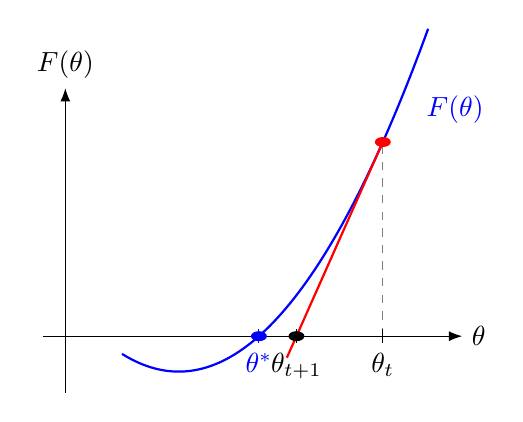
\begin{tikzpicture}[scale=0.9, xscale=1.6, >=Latex] 
                % --- Setup Definitions ---
                % Function: y = (x-1)^2 - 0.5. 
                % Initial Guess xt = 2.8
                \def\xt{2.8}              
                \def\yt{2.74}             % F(2.8) = (1.8)^2 - 0.5 = 2.74
                \def\xnext{2.038}         % 2.8 - 2.74/3.6 = 2.038...
                \def\xstar{1.707}         % True root
            
                % --- Axes ---
                \draw[->] (-0.2,0) -- (3.5,0) node[right] {$\theta$};
                \draw[->] (0,-0.8) -- (0,3.5) node[above] {$F(\theta)$};
            
                % --- Function Curve ---
                \draw[thick, blue, samples=100, domain=0.5:3.2] plot (\x, {(\x-1)*(\x-1) - 0.5});
                \node[blue, right] at (3.1, 3.2) {$F(\theta)$};
            
                % --- Current Guess theta_t ---
                \draw[dashed, gray] (\xt, 0) -- (\xt, \yt);
                \fill[red] (\xt, \yt) circle (2pt);
                \draw (\xt, 0.1) -- (\xt, -0.1) node[below] {$\theta_t$};
            
                % --- Tangent Line (Linearization) ---
                % Plain red line, no text
                \draw[red, thick, shorten >=-0.3cm] (\xt, \yt) -- (\xnext, 0);

                % --- Next Guess theta_{t+1} ---
                \fill[black] (\xnext, 0) circle (2pt);
                \draw (\xnext, 0.1) -- (\xnext, -0.1) node[below] {$\theta_{t+1}$};

                % --- True Root theta^* ---
                \fill[blue] (\xstar, 0) circle (2pt);
                \draw[blue] (\xstar, 0.1) -- (\xstar, -0.1) node[below] {$\theta^*$};
        \end{tikzpicture}
        \end{column}
    \end{columns}
\end{frame}

% Slide: Step 3 - Algorithm B (Gradient Descent)
\begin{frame}{Step 3: Gradient Descent (Minimization)}
\small
    \begin{itemize}
    \item Context: Used for Over-Identified systems ($M > K$) to minimize the Loss $\mathcal{L}(\theta)$, or when $K$ is too large for Newton.
    
    \item Relation to Newton's Method (Optimization):
    \begin{itemize}
        \item To minimize $\mathcal{L}$, Newton's update would use the \textit{Hessian} (Matrix of 2nd derivatives $\mathbf{H}$):
        $$ \theta_{t+1} = \theta_t - \mathbf{H}(\theta_t)^{-1} \nabla \mathcal{L}(\theta_t) $$
        \item Gradient Descent simplifies this by approximating the inverse Hessian with a scalar identity matrix $\alpha \mathbf{I}$ (where $\alpha$ is step size):
        $$ \mathbf{H}(\theta_t)^{-1} \approx \alpha \mathbf{I} \implies \theta_{t+1} = \theta_t - \alpha \nabla \mathcal{L}(\theta_t) $$
    \end{itemize}
    
    \item Implication:
    \begin{itemize}
        \item Newton jumps directly to the minimum of the local quadratic approximation (uses curvature info in $\mathbf{H}$).
        \item Gradient Descent takes small steps based on local slope only (ignores curvature).
    \end{itemize}
    \end{itemize}
\end{frame}




% Slide 9: Introduction to Neural Networks
\begin{frame}{Introduction to Neural Networks}
\begin{itemize}
    \item A Neural Network (NN) is a specific type of non-linear parameterization $\hat{V}(s; \theta)$. Unlike linear bases where $\hat{V} = \sum \theta_i \phi_i(s)$, NNs nest parameters inside non-linear activation functions.
    \item Specifically, a feedforward neural network (FFN, or Multilayer Perceptron (MLP)) has each of its layer $\ell$:
    $$ x_\ell = \sigma_\ell (W_\ell x_{\ell-1} + b_\ell) \quad \text{for } \ell = 1, \dots, L $$
    \begin{itemize}
        \item Parameters $\theta = \{W_\ell, b_\ell\}_{\ell=1}^L$. Weights $W$ and biases $b$.
        \item Activation Function $\sigma(\cdot)$: Non-linear function applied element-wise.
        \item Common choices for $\sigma$: ReLU ($\max(0,z)$), Tanh, Sigmoid, SiLU.
    \end{itemize}
\end{itemize}
\end{frame}


\begin{frame}{Visualization of Activation Functions}
    \begin{figure}
        \centering
        \includegraphics[width=0.6\textwidth]{Approximation_NN_Activations.png}
    \end{figure}
    Interactive visualization: \url{https://playground.tensorflow.org/}
\end{frame}




\begin{frame}{Universal Approximation Theorem}
    \small
    \vspace{0.2cm}
    \begin{block}{Theorem (Hornik et al., 1989; Cybenko, 1989)}
    Let $f(s)$ be any continuous function on a compact domain $S$. For any error tolerance $\epsilon > 0$, there exists a Neural Network $\hat{V}(s; \theta)$ with a single hidden layer and finite width $N$ such that:
    $$ \sup_{s \in S} | f(s) - \hat{V}(s; \theta) | < \epsilon $$
    \end{block}
    \begin{itemize}
        \item Implications:
        \begin{itemize}
            \item Universality (Density): This property is mathematically known as being "dense" in the function space. It simply means that Neural Networks are not restricted to specific shapes. Unlike linear models (planes) or low-order polynomials (smooth curves), an NN can approximate any valid economic function to any desired degree of accuracy.
            \item Existence vs Construction: The theorem guarantees that a solution (the optimal $\theta$) exists, but it does not tell us how to find it. Finding these parameters requires numerical optimization (e.g., Stochastic Gradient Descent).
        \end{itemize}
    \end{itemize}
\end{frame}

\begin{frame}{NN vs conventional approximators}
    \small

    \begin{itemize}
        \item Adaptive Basis vs Fixed Basis
        \begin{itemize}
            \item Polynomials (Fixed): You fix the shapes ($s, s^2, s^3$) ex-ante. To fit a kink or a specific curve, you often need hundreds of global terms.
            \item Neural Nets (Adaptive): The basis functions $\sigma(w s + b)$ contain parameters ($w, b$) inside the function. The network learns to shift and rotate the basis to put the "complexity" exactly where the function changes, and leaves the rest flat.
        \end{itemize}

        \item Beating the Curse of Dimensionality (Barron's Theorem)
        \begin{itemize}
            \item Conventional Methods: The error decays as $O(N^{-1/d})$. In high dimensions ($d$), you need exponentially more parameters to reduce error (filling the volume).
            \item Neural Networks: The error decays as $O(N^{-1/2})$. The rate is independent of the dimension $d$. 
            \item Intuition: NNs act like a Monte Carlo simulation. Instead of filling the entire grid, they sample the directions where the function varies the most. The error depends on the complexity of the target function, not the volume of the input space.
        \end{itemize}
    \end{itemize}
\end{frame}
% Slide 12a: Training Neural Networks - Connecting to the Framework
\begin{frame}{Training NNs: Optimization via General Framework}
    \small
    \vspace{0.3mm}
    Training a Neural Network is just a specific instance of our general numerical framework.
    \begin{itemize}
        \item Step 1 (Residual Function): Define the error at a single state $s$.
        \begin{itemize}
            \item The residual is the Bellman error: $R(s; \theta) = \hat{V}(s; \theta) - \mathcal{T}\hat{V}(s; \theta)$.
            \item Here $\hat{V}(s; \theta)$ is the Neural Network output.
        \end{itemize}
        
        \item Step 2 (Objective Function): Aggregate residuals (Method C: Least Squares).
        \begin{itemize}
            \item Since we are in the over-identified case ($M \gg K$), we minimize the Mean Squared Error over a set of sampled states:
            $$ \min_{\theta} \mathcal{L}(\theta) = \frac{1}{M} \sum_{i=1}^M \| R(s_i; \theta) \|^2 $$
            \item The sampling distribution $\mu(s)$ implicitly acts as the weighting function $w(s)$.
        \end{itemize}

        \item Step 3 (Solver Algorithm): Gradient Descent.
        \begin{itemize}
            \item We cannot use Newton-Raphson because the Jacobian is too large ($K \sim 10^5+$).
            \item Instead, we use First-Order methods: $\theta_{t+1} = \theta_t - \alpha \nabla_\theta \mathcal{L}(\theta)$.
        \end{itemize}
    \end{itemize}
\end{frame}

% Slide 12b: The Key Enabler - Automatic Differentiation
\begin{frame}{Training NNs: Automatic Differentiation}
    \small
    \begin{itemize}
        \item A Neural Network is a nested chain of non-linear functions:
        $$ \hat{V}(s) = \sigma(W_L \dots \sigma(W_1 s + b_1) \dots ) $$
        Deriving gradients $\frac{\partial \mathcal{L}}{\partial W_1}$ by hand (symbolic differentiation) is error-prone and impossible for deep networks.
        
        \item Automatic Differentiation (Auto-diff):
        \begin{itemize}
            \item Modern frameworks (PyTorch, TensorFlow) build a "Computational Graph" as you calculate the residual $R(s; \theta)$.
            \item They apply the Chain Rule automatically from the output back to the inputs (Backpropagation).
            \item Result: We get exact gradients $\nabla_\theta \mathcal{L}$ with computational cost proportional to just one forward pass.
        \end{itemize}

        \item Simple Example: $y = (w \cdot x)^2$
        \begin{itemize}
            \item Forward (Graph Construction): 
            $ \text{Input } w, x \xrightarrow{z = w \cdot x} \text{Node } z \xrightarrow{y = z^2} \text{Output } y $
            \item Backward (Gradient Calculation):
            $ \frac{\partial y}{\partial w} = \underbrace{\frac{\partial y}{\partial z}}_{2z} \cdot \underbrace{\frac{\partial z}{\partial w}}_{x} = 2(wx) \cdot x $
        \end{itemize}
    \end{itemize}
\end{frame}

% Slide 12c: Training Neural Networks - Stochastic Gradient Descent
\begin{frame}{Training NNs: Stochastic Gradient Descent (SGD)}
    \small
    With Auto-diff handling the gradient computation, we use SGD to handle the large data scale.
    
    \begin{itemize}
        \item The Problem with Full Gradient Descent:
        \begin{itemize}
            \item Computing $\nabla_\theta \mathcal{L}$ requires summing errors over all $M$ states (e.g., $M=10^6$). This is too slow per step.
        \end{itemize}
        
        \item The SGD Solution (Mini-Batch):
        \begin{itemize}
            \item Sample a small batch $B \subset \{s_1, \dots, s_M\}$ (e.g., size 64).
            \item Estimate the gradient using only this batch:
            $$ \mathbf{g}_{batch} = \nabla_\theta \frac{1}{|B|} \sum_{s \in B} \| R(s; \theta) \|^2 $$
            \item Update: $\theta \leftarrow \theta - \alpha \cdot \mathbf{g}_{batch}$
        \end{itemize}
        
        \item Summary of the Training Loop:
        \begin{enumerate}
            \item Sample batch $B$.
            \item Forward Pass: Compute Residuals $R(s)$.
            \item Backward Pass (Auto-diff): Compute Gradients $\nabla_\theta \mathcal{L}$.
            \item Optimizer Step: Update $\theta$ using SGD.
        \end{enumerate}
    \end{itemize}
\end{frame}




\end{document}